\documentclass[aspectratio=169]{beamer}

\usepackage{ccicons}
\usepackage{fontspec}
\usepackage{import}
\usepackage{listings}
\usepackage{tikz}

\subimport{../}{colors.tex}

\usetikzlibrary{
  arrows,
  arrows.meta,
  automata,
  backgrounds,
  calc,
  chains,
  decorations.pathreplacing,
  fit,
  matrix,
  overlay-beamer-styles,
  positioning,
  shapes,
  tikzmark,
}
\usetikzmarklibrary{listings}

\hypersetup{
  colorlinks=true,
  urlcolor=uclablue,
}

\setbeamercolor{frametitle}{fg=primarycolor}
\setbeamercolor{structure}{fg=primarycolor}
\setbeamercolor{enumerate item}{fg=black}
\setbeamercolor{itemize item}{fg=black}
\setbeamercolor{itemize subitem}{fg=black}

\setbeamersize{text margin left=26.6mm}
\addtolength{\headsep}{2mm}

\setbeamertemplate{navigation symbols}{}
\setbeamertemplate{headline}{}
\setbeamertemplate{footline}{}
\setbeamertemplate{itemize item}{\color{black}}
\setbeamertemplate{itemize items}[circle]

\setbeamertemplate{footline}{
  \begin{tikzpicture}[remember picture,
                      overlay,
                      shift={(current page.south west)}]
    \node [black!50, inner sep=2mm, anchor=south east]
          at (current page.south east) {\footnotesize \insertframenumber};
  \end{tikzpicture}
}

\setsansfont{Overpass}[Scale=MatchLowercase]
\setmonofont{Overpass Mono}[Scale=MatchLowercase]

\makeatletter
\newcommand\version[1]{\renewcommand\@version{#1}}
\newcommand\@version{}
\def\insertversion{\@version}

\newcommand\lecturenumber[1]{\renewcommand\@lecturenumber{#1}}
\newcommand\@lecturenumber{}
\def\insertlecturenumber{\@lecturenumber}
\makeatother

\setbeamertemplate{title page}
{
  \begin{tikzpicture}[remember picture,
                      overlay,
                      shift={(current page.south west)},
                      background rectangle/.style={fill=uclablue},
                      show background rectangle]
    \node [anchor=west, align=left, inner sep=0, text=white]
          (lecturenumber) at (\paperwidth / 6, \paperheight * 3 / 4)
          {\Large Lecture \insertlecturenumber};
    \node [inner sep=0, align=left, text=white, node distance=0,
           above left=of lecturenumber, anchor=south west, yshift=2mm]
          {\Large CS 111: Operating System Principles};
    \node (title) [inner sep=0, anchor=west, align=right, text=white]
          at (\paperwidth / 6, \paperheight / 2)
          {{\bfseries \Huge \inserttitle{}}};
    \node [inner sep=0, align=right, text=white, node distance=0,
           below right=of title, anchor=north east, yshift=-1mm]
          {{\footnotesize \ttfamily \insertversion}};
    \node [inner sep=0, text=white, align=left, anchor=west]
          (author) at (\paperwidth / 6, \paperheight / 4)
          {\insertauthor};
    \node [text=white, inner sep=0, align=left, node distance=0,
           below left=of author, anchor=north west, yshift=-2mm]
          {\insertdate};
    \node [align=right, anchor=south east, inner sep=2mm, text=white]
          (license) at (\paperwidth, 0)
          {\footnotesize This  work is licensed under a
           \href{http://creativecommons.org/licenses/by-sa/4.0/}
                {\color{uclagold} Creative Commons Attribution-ShareAlike 4.0
                 International License}};
    \node [text=white, inner sep=0, align=right, node distance=0,
           above right=of license, anchor=south east, xshift=-2mm]
          {\Large \ccbysa};
  \end{tikzpicture}
}

\tikzset{
  >=Straight Barb[],
  shorten >=1pt,
  initial text=,
}

\lstset{
  basicstyle=\footnotesize\ttfamily,
}


\lecturenumber{10}
\title{Page Tables}
\version{1.0.1}
\author{Jon Eyolfson}
\date{April 20, 2021}

\begin{document}
  \begin{frame}[plain, noframenumbering]
    \titlepage
  \end{frame}

  \begin{frame}
    \frametitle{Virtualization Fools Something into Thinking it Has All Resources}

    \begin{columns}[c]
      \column{0.5\textwidth}
      \flushright
    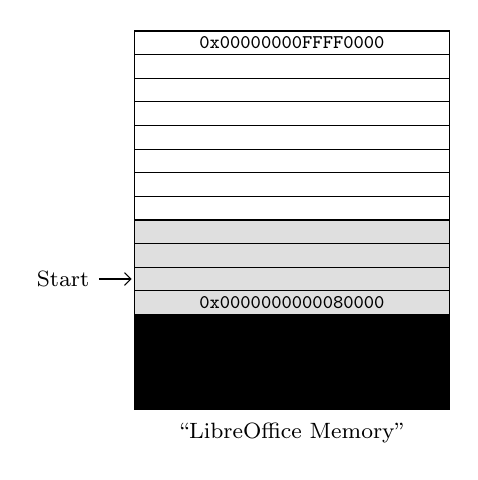
\begin{tikzpicture}
      \node [align=center] at (2, 0) {\footnotesize ``LibreOffice Memory''};
      \draw [fill=black] (0, 0.3) rectangle (4, 1.5);
      \draw [fill=black!12.5] (0, 1.5) rectangle (4, 2.7);
      \node [align=center] at (2, 1.65) {\scriptsize \ttfamily 0x0000000000080000};
      \node [align=center] at (2, 4.95) {\scriptsize \ttfamily 0x00000000FFFF0000};
      \foreach \i in {1, ..., 16}
      {
        \draw (0, 0.3 * \i) rectangle (4, \i * 0.3 + 0.3);
      }

      \draw [->] (-0.45, 1.95) -- (0, 1.95) node [pos=0, anchor=east] {\footnotesize Start};
    \end{tikzpicture}
      \column{0.5\textwidth}
      \flushleft
    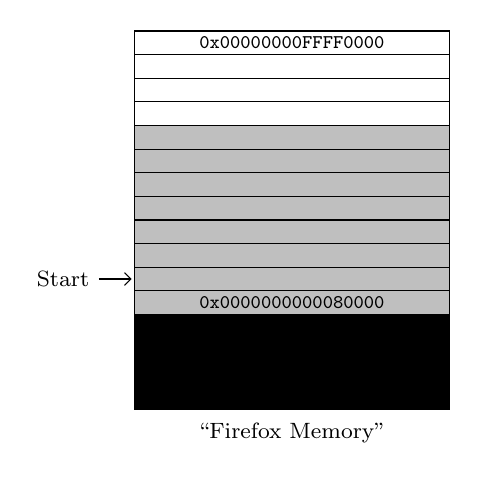
\begin{tikzpicture}
      \node [align=center] at (2, 0) {\footnotesize ``Firefox Memory''};
      \draw [fill=black] (0, 0.3) rectangle (4, 1.5);
      \draw [fill=black!25] (0, 1.5) rectangle (4, 3.9);
      \node [align=center] at (2, 1.65) {\scriptsize \ttfamily 0x0000000000080000};
      \node [align=center] at (2, 4.95) {\scriptsize \ttfamily 0x00000000FFFF0000};
      \foreach \i in {1, ..., 16}
      {
        \draw (0, 0.3 * \i) rectangle (4, \i * 0.3 + 0.3);
      }

      \draw [->] (-0.45, 1.95) -- (0, 1.95) node [pos=0, anchor=east] {\footnotesize Start};
    \end{tikzpicture}
    \end{columns}
  \end{frame}

  \begin{frame}
    \frametitle{Virtual Memory Checklist}

    \begin{itemize}
      \item [$\square$] Multiple processes must be able to co-exist
      \item [$\square$] Processes are not aware they are sharing physical memory
      \item [$\square$] Processes cannot access each others data (unless allowed explicitly)
      \item [$\square$] Performance close to using physical memory
      \item [$\square$] Limit the amount of fragmentation (wasted memory)
    \end{itemize}
  \end{frame}

  \begin{frame}
    \frametitle{Memory Management Unit (MMU)}

    Maps virtual address to physical address

    \hspace{2em} Also checks permissions

    \vspace{2em}

    One technique is to divide memory up into fixed-size pages (typically 4096 bytes)

    \hspace{2em} A page in virtual memory is called a page

    \hspace{2em} A page in physical memory is called a frame
  \end{frame}

  \begin{frame}
    \frametitle{Segmentation or Segments are Coarse Grained}

    Divide the virtual address space into segments for: code, data, stack, and heap

    \hspace{2em} Note: this looks like an ELF file, large sections of memory with permissions

    \vspace{2em}

    Each segment is a variable size, and can be dynamically resized

    \hspace{2em} This is an old legacy technique that's no longer used

    \vspace{2em}

    Segments can be large and very costly to relocate

    \hspace{2em} It also leads to fragmentation (gaps of unused memory)

    \vspace{2em}

    No longer used in modern operating systems
  \end{frame}

  \begin{frame}
    \frametitle{Segmentation Details}

    Each segment contains a: base, limit, and permissions

    \hspace{2em} You get a physical address by using: \texttt{segment selector:offset}

    \vspace{2em}

    The MMU checks that your offset is within the limit (size)

    \hspace{2em} If it is, it calculates base + offset, and does permission checks

    \hspace{4em} Otherwise, it's a segmentation fault

    \vspace{2em}

    For example 0x1:0xFF with segment 0x1 base = 0x2000, limit = 0x1FF

    \hspace{2em} Translates to 0x20FF

    \vspace{2em}

    Note: Linux sets every base to 0, and limit to the maximum amount
  \end{frame}

  %% \begin{frame}
  %%   \begin{tikzpicture}[
  %%     start chain=1 going right,
  %%     start chain=2 going right,
  %%     cat/.style={draw, node distance=0pt, minimum width=6em},
  %%     num/.style={node distance=0pt, font=\scriptsize},
  %%   ]
  %%     \node [cat, fill=black!30, on chain=1] {Unused};
  %%     \node [cat, on chain=1] (index) {Index};
  %%     \node [cat, on chain=1] (offset) {Offset};

  %%     \node [num, above left=of index, anchor=south west] {38};
  %%     \node [num, above right=of index, anchor=south east] {12};

  %%     \node [num, above left=of offset, anchor=south west] {11};
  %%     \node [num, above right=of offset, anchor=south east] {0};
  %%   \end{tikzpicture}
  %% \end{frame}

  \begin{frame}
    \frametitle{You Typically Do Not Use All 64 Virtual Address Bits}

    CPUs may have different levels of virtual addresses you can use

    \hspace{2em} Implementation ideas are the same

    \vspace{2em}

    We'll assume a 39 bit virtual address space used by RISC-V and other
    architectures

    \hspace{2em} Allows for 512 GiB of addressable memory (called Sv39)

    \vspace{2em}

    Implemented with a page table indexed by Virtual Page Number (VPN)

    \hspace{2em} Looks up the Physical Page Number (PPN)
  \end{frame}

  \begin{frame}
    \frametitle{The Page Table Translates Virtual to Physical Addresses}

    \begin{center}
      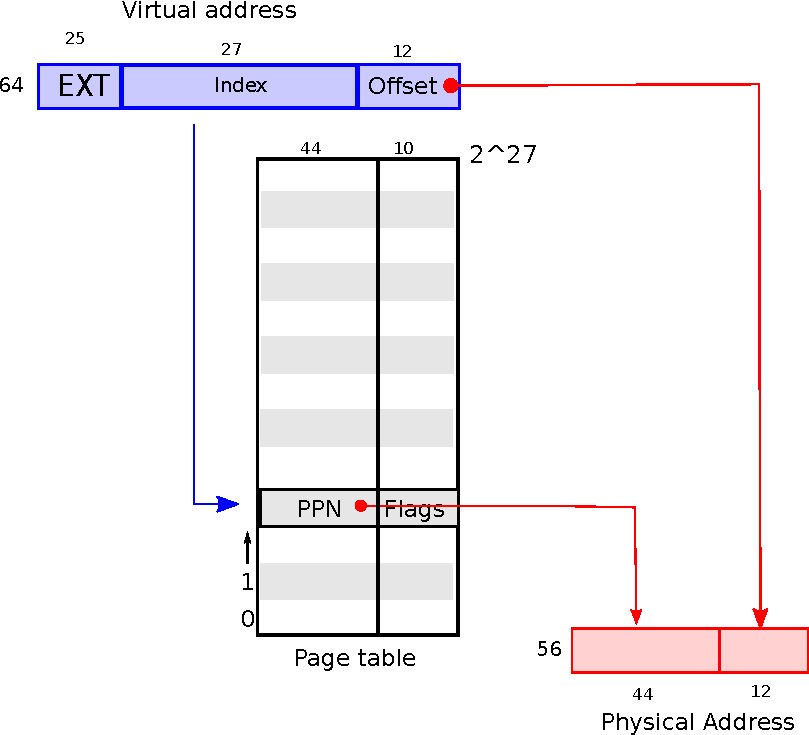
\includegraphics[scale=0.5]{riscv_address.pdf}
    \end{center}

    © MIT \url{https://github.com/mit-pdos/xv6-riscv-book/}
  \end{frame}

  \begin{frame}
    \frametitle{The Kernel Handles Translating Virtual Addresses}

    Considering the following page table:

    \begin{center}
    {\ttfamily
    \begin{tabular}{ll}
      VPN  & PPN  \\
      0x0 & 0x1 \\
      0x1 & 0x4 \\
      0x2 & 0x3 \\
      0x3 & 0x7 \\
    \end{tabular}}
    \end{center}

    We would get the following virtual $\rightarrow$ physical address translations:

    \begin{center}
    \texttt{0x0AB0} $\rightarrow$ \texttt{0x1AB0}
    
    \texttt{0x1FA0} $\rightarrow$ \texttt{0x4FA0}

    \texttt{0x2884} $\rightarrow$ \texttt{0x3884}

    \texttt{0x32D0} $\rightarrow$ \texttt{0x72D0}
    \end{center}
  \end{frame}

  \begin{frame}
    \frametitle{Page Translation Example Problem}

    Assume you have a 8-bit virtual address, 10-bit physical address

    \hspace{2em} and each page is 64 bytes

    \begin{itemize}
      \item How many virtual pages are there? \onslide<2->{$\mathsf{\frac{2^8}{2^6} = 4}$}
      \item How many physical pages are there? \onslide<2->{$\mathsf{\frac{2^{10}}{2^6} = 16}$}
      \item How many entries are in the page table? \onslide<2->{$\mathsf{4}$}
      \item Given the page table is \texttt{{[0x2, 0x5, 0x1, 0x8]}}

            \hspace{2em} what's the physical address of \texttt{0xF1}?

            \onslide<2->{\texttt{0x231}}
    \end{itemize}
  \end{frame}

  \begin{frame}
    \frametitle{The Page Table Entry (PTE) Also Stores Flags in the Lower Bits}

    \begin{center}
      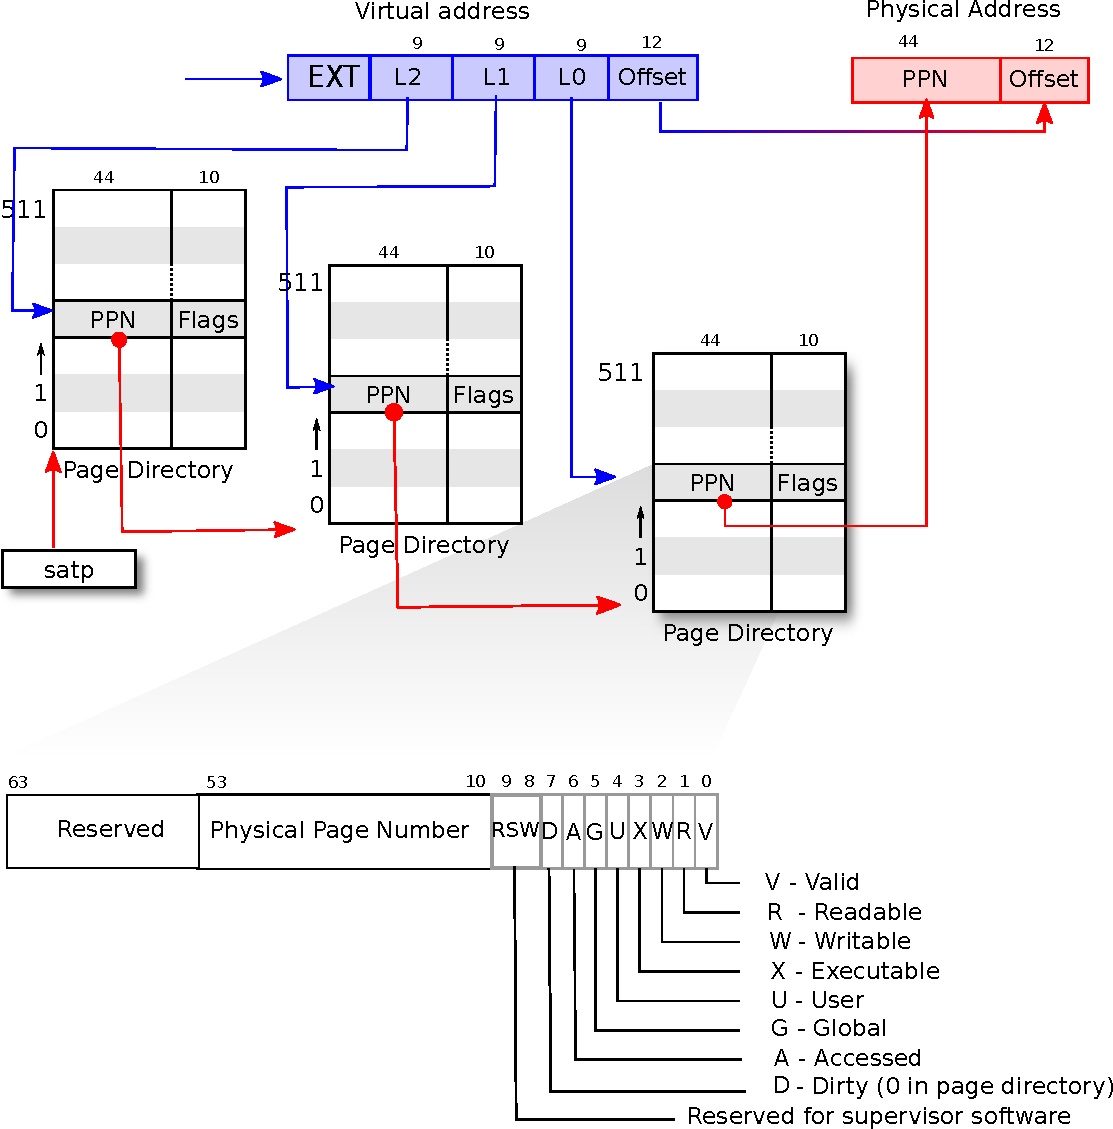
\includegraphics[scale=0.5, clip, trim=0cm 0cm 0cm 13cm]{riscv_pagetable.pdf}
    \end{center}

    © MIT \url{https://github.com/mit-pdos/xv6-riscv-book/}

    \vspace{2em}

    The MMU which uses the page table checks these flags

    \hspace{2em} We'll focus on the first 5 flags
  \end{frame}

  \begin{frame}
    \frametitle{Each Process Gets Its Own Virtual Address Space}

    \begin{center}
      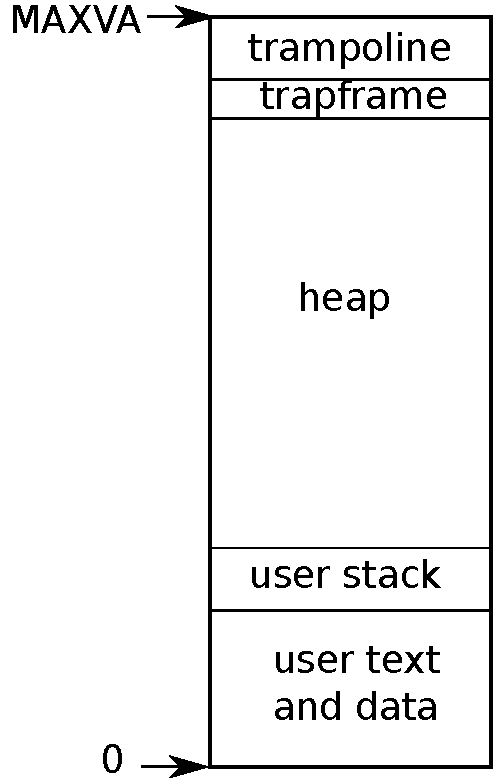
\includegraphics[scale=0.4]{as.pdf}
    \end{center}

    © MIT \url{https://github.com/mit-pdos/xv6-riscv-book/}
  \end{frame}

  \begin{frame}
    \frametitle{Each Process Gets Its Own Page Table}

    When you \texttt{fork} a process, it will copy the page table from the parent

    \hspace{2em} Turn off the write permission so the kernel can implement
    copy-on-write

    \vspace{2em}

    The problem is there are $\mathsf{2^{27}}$ entries in the page table, each
    one is 8 bytes

    \hspace{2em} This means the page table would be 1 GiB

    \vspace{2em}

    Note that RISC-V translates a 39-bit virtual to a 56-bit physical address

    \hspace{2em} It has 10 bits to spare in the PTE and could expand

    \hspace{2em} Page size is 4096 bytes (size of offset field)
  \end{frame}

  \begin{frame}
    \frametitle{You May Be Thinking That Seems Like A Lot of Work}

    In Lab 1, we're doing a \texttt{fork} followed by \texttt{exec} why do we
    need to copy the page tables?

    \vspace{2em}

    We don't! There's a system call for that --- \texttt{vfork}

    \vspace{2em}

    \texttt{vfork} shares all memory with the parent

    \hspace{2em} It's undefined behavior to modify anything

    \vspace{2em}

    Only used in very performance sensitive programs
  \end{frame}

  \begin{frame}
    \frametitle{Multi-Level Page Tables Save Space for Sparse Allocations}

    \begin{center}
      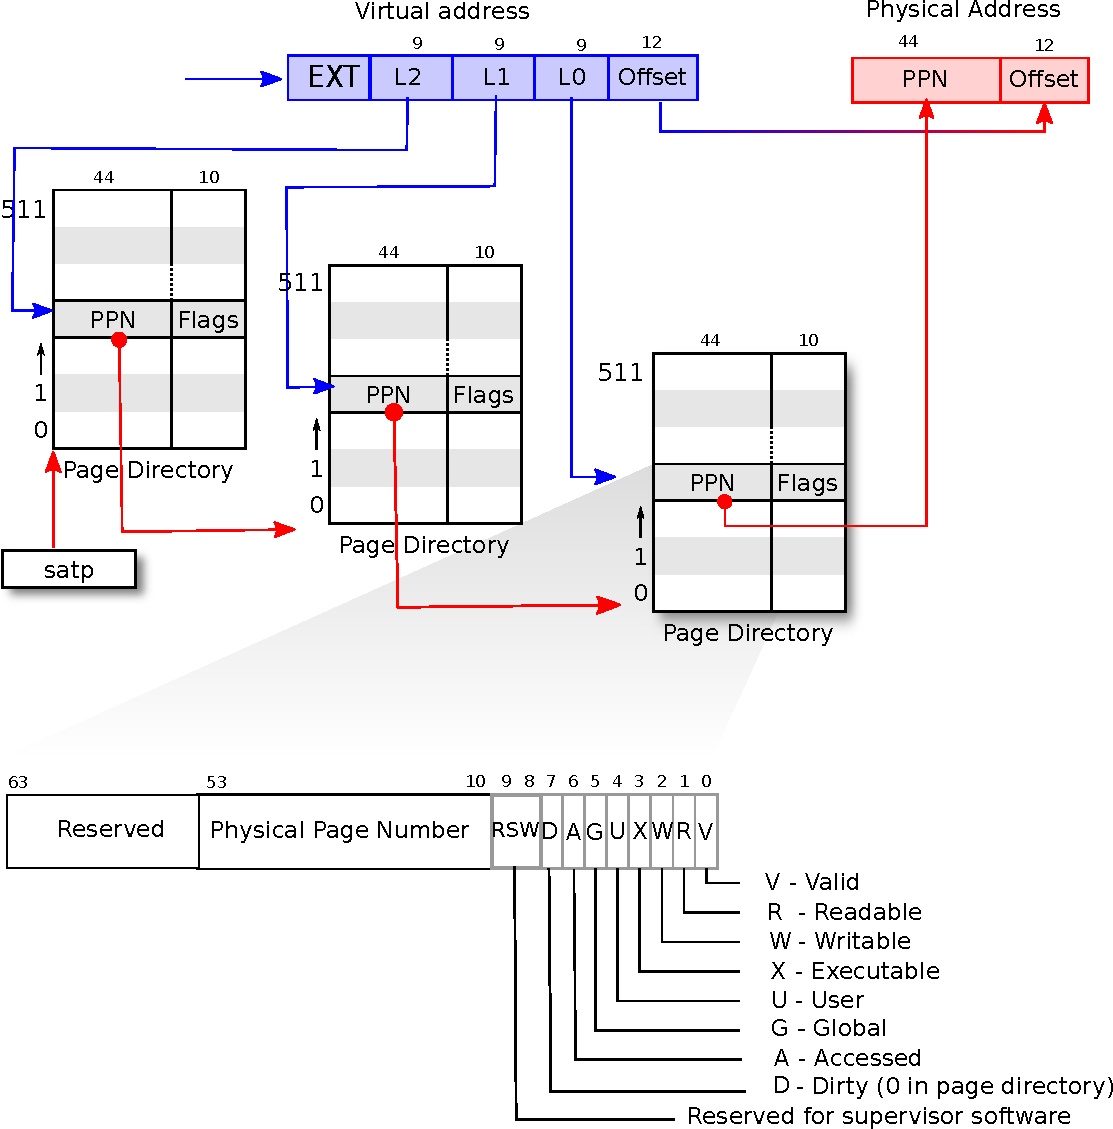
\includegraphics[scale=0.5, clip, trim=0cm 8cm 0cm 0cm]{riscv_pagetable.pdf}
    \end{center}

    © MIT \url{https://github.com/mit-pdos/xv6-riscv-book/}
  \end{frame}

  \begin{frame}
    \frametitle{For RISC-V Each Level Occupies One Page}

    There are 512 ($\mathsf{2^9}$) entries of 8 bytes($\mathsf{2^3}$) each, which is 4096 bytes

    \vspace{2em}

    The PTE for L(N) points to the page table for L(N-1)

    \vspace{2em}

    You follow these page tables until L0 and that contains the \texttt{PPN}
  \end{frame}

  \begin{frame}
    \frametitle{Consider Just One Additional Level}

    Assume our process uses just one virtual address at \texttt{0x3FFFF008}

    \hspace{2em} or \texttt{0b11\_1111\_1111\_1111\_1111\_0000\_0000\_1000}

    \hspace{2em} or \texttt{0b111111111\_111111111\_000000001000}

    \vspace{2em}

    We'll just consider a 30-bit virtual address with a page size of 4096 bytes

    \hspace{2em} We would need a 2 MiB page table if we only had one ($\mathsf{2^{18} \times 2^{3}}$)

    \vspace{2em}

    Instead we have a 4 KiB L1 page table ($\mathsf{2^9 \times 2^{3}}$) and a 4 KiB L0 page table

    \hspace{2em} Total of 8 KiB instead of 2 MiB

    \vspace{2em}

    Note: worst case if we used all virtual addresses we would consume 2 MiB + 4 KiB
  \end{frame}

  \begin{frame}
    \frametitle{Translating \texttt{3FFFF008} with 2 Page Tables}

    Consider the L1 table with the entry:

    \begin{center}
    {\ttfamily
    \begin{tabular}{rl}
      Index & PPN \\
      511   & 0x8 \\
    \end{tabular}}
    \end{center}
      
    Consider the L0 table located at \texttt{0x8000} with the entry:

    \begin{center}
    {\ttfamily
    \begin{tabular}{rl}
      Index & PPN \\
      511   & 0xCAFE \\
    \end{tabular}}
    \end{center}
    
    The final translated physical address would be: \texttt{0xCAFE008}
  \end{frame}

  \begin{frame}
    \frametitle{Processes Use A Register Like \texttt{satp} to Set the Root Page Table}

    \begin{center}
      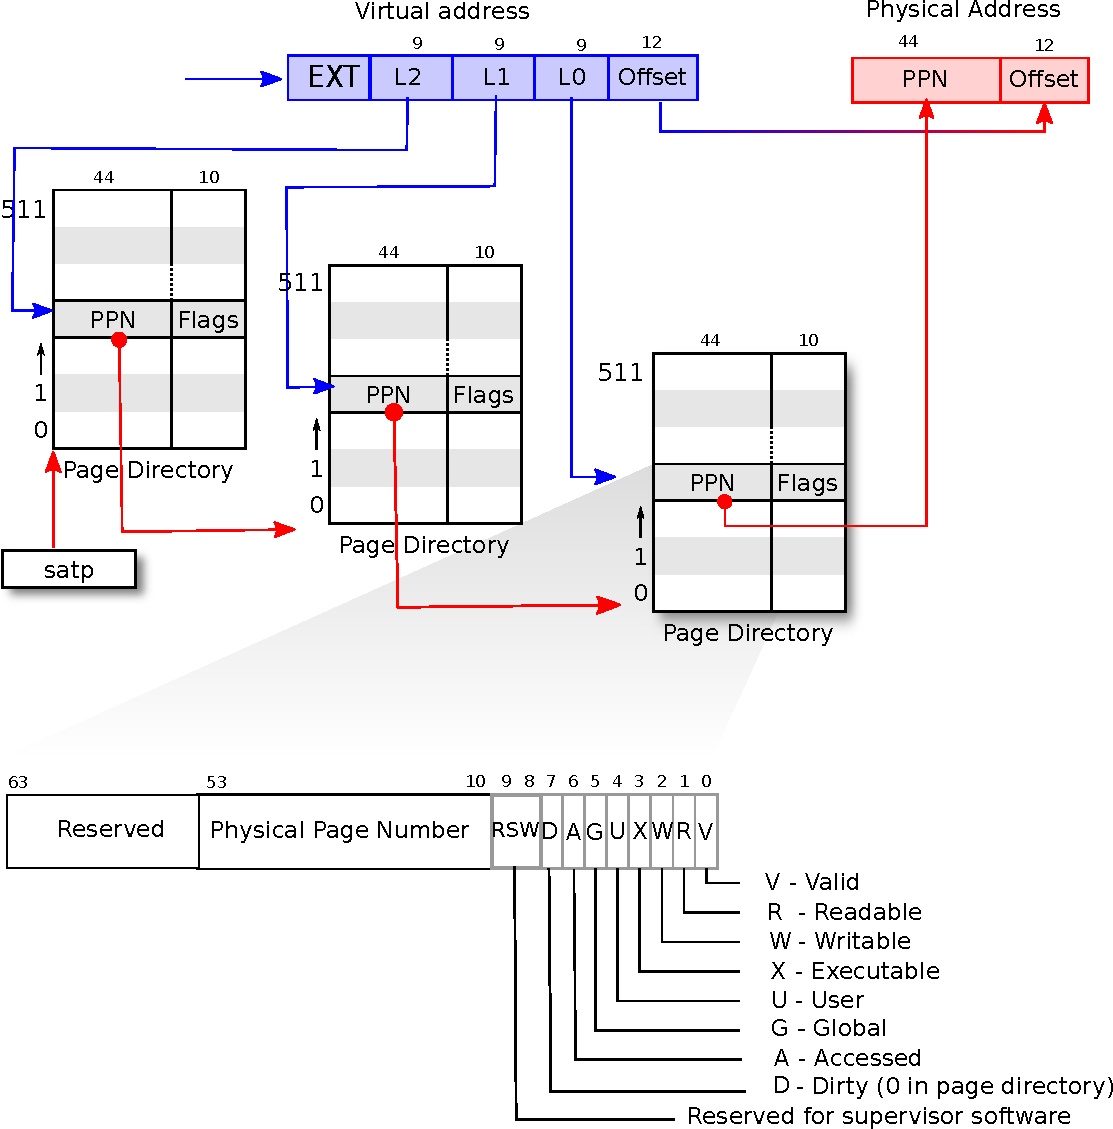
\includegraphics[scale=0.5, clip, trim=0cm 8cm 0cm 0cm]{riscv_pagetable.pdf}
    \end{center}

    © MIT \url{https://github.com/mit-pdos/xv6-riscv-book/}
  \end{frame}

  \begin{frame}
    \frametitle{Page Allocation Uses A Free List}

    Given physical pages, the operating system maintains a free list (linked list)

    \vspace{2em}

    The unused pages themselves contain the \texttt{next} pointer in the free list

    \hspace{2em} Physical memory gets initialized at boot

    \vspace{2em}

    To allocate a page, you remove it from the free list

    \hspace{2em} To deallocate a page you add it back to the free list
  \end{frame}

  \begin{frame}
    \frametitle{Using the Page Tables for Every Memory Access is Slow}

    We need to follow pointers across multiple levels of page tables!

    \vspace{2em}

    We'll likely access the same page multiple times (close to the first access time)

    \vspace{2em}

    A process may only need a few VPN $\rightarrow$ PPN mappings at a time

    \vspace{2em}

    Our solution is another computer science classic: caching
  \end{frame}

  \begin{frame}
    \frametitle{A Translation Look-Aside Buffer (TLB) Caches Virtual Addresses}

    \begin{center}
    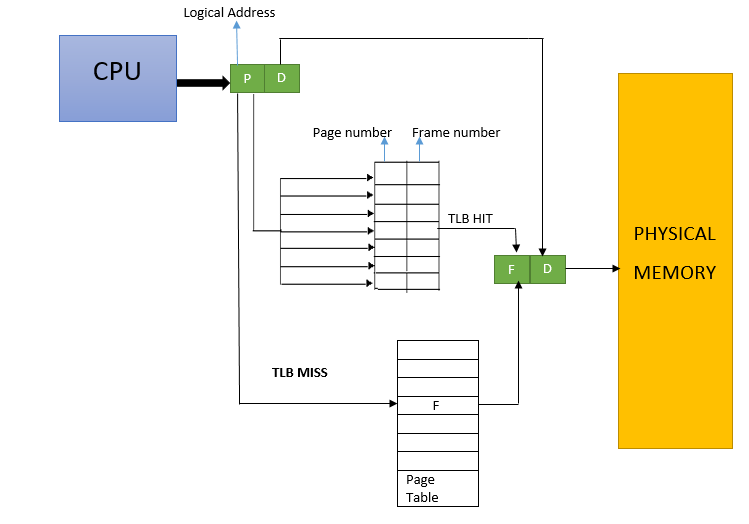
\includegraphics[scale=0.45]{tlb.png}
    \end{center}

    ``Working flow of a TLB'' by Aravind Krishna is licensed under CC BY-SA 4.0
  \end{frame}

  \begin{frame}
    \frametitle{Effective Access Time (EAT)}

    Assume a single page table (there's only one additional memory access in the page table)

    \vspace{2em}

    $\mathsf{TLB\_Hit\_Time = TLB\_Search + Mem}$

    $\mathsf{TLB\_Miss\_Time = TLB\_Search + 2 \times Mem}$

    $\mathsf{EAT = \alpha \times TLB\_Hit\_Time + (1 - \alpha) \times TLB\_Miss\_Time}$

    \vspace{2em}

    If $\mathsf{\alpha = 0.8}$, $\mathsf{TLB\_Search = 10\ ns}$, and memory accesses take 100 ns, calculate EAT

    \hspace{2em} $\mathsf{EAT = 0.8 \times 110\ ns + 0.2 \times 210\ ns}$

    \hspace{2em} $\mathsf{EAT = 130\ ns}$
  \end{frame}

  \begin{frame}
    \frametitle{Context Switches Require Handling the TLB}

    You can either flush the cache, or attach a process ID to the TLB

    \vspace{2em}

    Most implementation just flush the TLB

    \hspace{2em} RISC-V uses a \texttt{sfence.vma} instruction to flush the TLB

    \vspace{2em}

    On x86 loading the base page table will also flush the TLB

  \end{frame}

  \begin{frame}
    \frametitle{How Many Levels Do I Need?}

    Assume we have a 32-bit virtual address with a page size of 4096 bytes

    \hspace{2em} and a PTE size of 4 bytes

    \vspace{2em}

    We want each page table to fit into a single page

    \hspace{2em} Find the number of PTEs we could have in a page ($\mathsf{2^{10}}$)

    \hspace{4em} $\mathsf{log_2(\# PTEs\ per\ Page)}$ is the number of bits to index a page table

    \vspace{2em}

    $\mathsf{\# Levels = \lceil \frac{Virtual\ Bits - Offset\ Bits}{Index\ Bits} \rceil}$

    \vspace{2em}

    \onslide<2->{$\mathsf{\# Levels = \lceil \frac{32 - 12}{10} \rceil = 2}$}
  \end{frame}

  \begin{frame}[fragile]
    \frametitle{TLB Testing}

    Check out \texttt{lecture-10/test-tlb}

    \hspace{2em} (you may need to \texttt{git submodule update --init --recursive})

    \vspace{2em}

    \texttt{./test-tlb <size> <stride>}

    \hspace{2em} Creates a <size> memory allocation and acccesses it every <stride> bytes

    \vspace{2em}

    Results from my laptop:

    \begin{lstlisting}
> ./test-tlb 4096 4        
  1.93ns (~7.5 cycles)
> ./test-tlb 536870912 4096
155.51ns (~606.5 cycles)
> ./test-tlb 16777216 128  
 14.78ns (~57.6 cycles)
    \end{lstlisting}
  \end{frame}

  \begin{frame}
    \frametitle{Use \texttt{sbrk} for Userspace Allocation}

    This call grows or shrinks your heap (the stack has a set limit)

    \vspace{2em}

    For growing, it'll grab pages from the free list to fulfill the request

    \hspace{2em} The kernel sets \texttt{PTE\_V} (valid) and other permissions

    \vspace{2em}

    In memory allocators this is difficult to use, you'll rarely shrink the heap

    \hspace{2em} It'll stay claimed by the process, and the kernel cannot free
    pages

    \vspace{2em}

    Memory allocators use \texttt{mmap} to bring in large blocks of virtual
    memory
  \end{frame}

  \begin{frame}
    \frametitle{The Kernel Initializes the Processs' Address Space (and Stack)}

    \begin{center}
      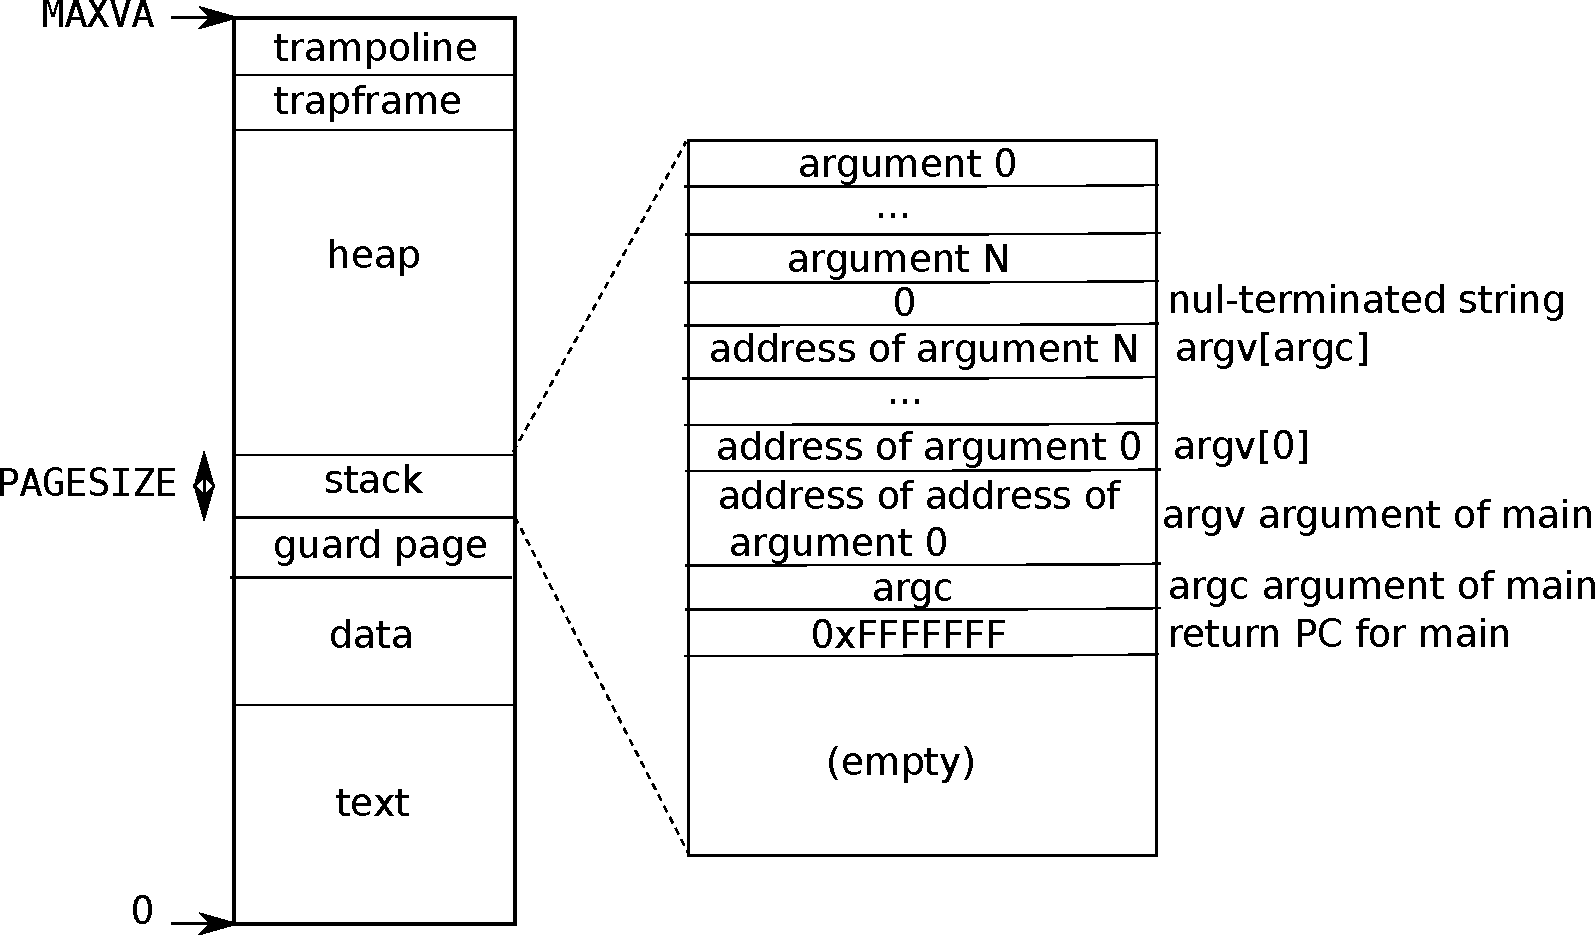
\includegraphics[scale=0.35]{processlayout.pdf}
    \end{center}

    © MIT \url{https://github.com/mit-pdos/xv6-riscv-book/}
  \end{frame}

  \begin{frame}
    \frametitle{A Trampoline is A Fixed Virtual Address Set by the Kernel}

    It allows the process to access kernel data without using
    a system call

    \vspace{2em}

    The guard page will generate an exception if accessed meaning stack overflow

    \vspace{2em}

    A trap is anytime special handler code runs:
    \begin{itemize}
      \item System call
      \item Exception
      \item Interrupt (e.g timer)
    \end{itemize}
  \end{frame}

  \begin{frame}
    \frametitle{Page Faults Allow the Operating System to Handle Virtual Memory}

    Page faults are a type of exception for virtual memory access

    \hspace{2em} Generated if it cannot find a translation, or permission check fails

    \vspace{2em}

    This allows the operating system to handle it

    \hspace{2em} We could lazily allocate pages, implement copy-on-write, or swap to disk
  \end{frame}

  \begin{frame}
    \frametitle{Page Tables Translate Virtual to Physical Addresses}

    The MMU is the hardware that uses page tables, which may:
    \begin{itemize}
      \item Be a single large table (wasteful, even for 32-bit machines)
      \item Be a multi-level to save space for sparse allocations
      \item Use the kernel allocate pages from a free list
      \item Use a TLB to speed up memory accesses
    \end{itemize}
  \end{frame}
\end{document}
